\documentclass[]{article}
\usepackage{amsfonts, amssymb, amsmath}
\usepackage{float}
\usepackage{graphicx}

\title{Question 12.13.3.1}
\author{Anupama Kulshreshtha \\ EE22BTECH11009}
\date{}
\begin{document}
\maketitle
\providecommand{\pr}[1]{\ensuremath{\Pr\left(#1\right)}}
\providecommand{\prt}[2]{\ensuremath{p_{#1}^{\left(#2\right)} }}        % own macro for this question
\providecommand{\qfunc}[1]{\ensuremath{Q\left(#1\right)}}
\providecommand{\sbrak}[1]{\ensuremath{{}\left[#1\right]}}
\providecommand{\lsbrak}[1]{\ensuremath{{}\left[#1\right.}}
\providecommand{\rsbrak}[1]{\ensuremath{{}\left.#1\right]}}
\providecommand{\brak}[1]{\ensuremath{\left(#1\right)}}
\providecommand{\lbrak}[1]{\ensuremath{\left(#1\right.}}
\providecommand{\rbrak}[1]{\ensuremath{\left.#1\right)}}
\providecommand{\cbrak}[1]{\ensuremath{\left\{#1\right\}}}
\providecommand{\lcbrak}[1]{\ensuremath{\left\{#1\right.}}
\providecommand{\rcbrak}[1]{\ensuremath{\left.#1\right\}}}
\newcommand{\sgn}{\mathop{\mathrm{sgn}}}
\providecommand{\abs}[1]{\left\vert#1\right\vert}
\providecommand{\res}[1]{\Res\displaylimits_{#1}} 
\providecommand{\norm}[1]{\left\lVert#1\right\rVert}
%\providecommand{\norm}[1]{\lVert#1\rVert}
\providecommand{\mtx}[1]{\mathbf{#1}}
\providecommand{\mean}[1]{E\left[ #1 \right]}
\providecommand{\cond}[2]{#1\middle|#2}
\providecommand{\fourier}{\overset{\mathcal{F}}{ \rightleftharpoons}}
\newenvironment{amatrix}[1]{%
  \left(\begin{array}{@{}*{#1}{c}|c@{}}
}{%
  \end{array}\right)
}
%\providecommand{\hilbert}{\overset{\mathcal{H}}{ \rightleftharpoons}}
%\providecommand{\system}{\overset{\mathcal{H}}{ \longleftrightarrow}}
	%\newcommand{\solution}[2]{\textbf{Solution:}{#1}}
\newcommand{\solution}{\noindent \textbf{Solution: }}
\newcommand{\cosec}{\,\text{cosec}\,}
\providecommand{\dec}[2]{\ensuremath{\overset{#1}{\underset{#2}{\gtrless}}}}
\newcommand{\myvec}[1]{\ensuremath{\begin{pmatrix}#1\end{pmatrix}}}
\newcommand{\mydet}[1]{\ensuremath{\begin{vmatrix}#1\end{vmatrix}}}
\newcommand{\myaugvec}[2]{\ensuremath{\begin{amatrix}{#1}#2\end{amatrix}}}
\providecommand{\rank}{\text{rank}}
\providecommand{\pr}[1]{\ensuremath{\Pr\left(#1\right)}}
\providecommand{\qfunc}[1]{\ensuremath{Q\left(#1\right)}}
	\newcommand*{\permcomb}[4][0mu]{{{}^{#3}\mkern#1#2_{#4}}}
\newcommand*{\perm}[1][-3mu]{\permcomb[#1]{P}}
\newcommand*{\comb}[1][-1mu]{\permcomb[#1]{C}}
\providecommand{\qfunc}[1]{\ensuremath{Q\left(#1\right)}}
\providecommand{\gauss}[2]{\mathcal{N}\ensuremath{\left(#1,#2\right)}}
\providecommand{\diff}[2]{\ensuremath{\frac{d{#1}}{d{#2}}}}
\providecommand{\myceil}[1]{\left \lceil #1 \right \rceil }
\newcommand\figref{Fig.~\ref}
\newcommand\tabref{Table~\ref}
\newcommand{\sinc}{\,\text{sinc}\,}
\newcommand{\rect}{\,\text{rect}\,}
%%
%	%\newcommand{\solution}[2]{\textbf{Solution:}{#1}}
%\newcommand{\solution}{\noindent \textbf{Solution: }}
%\newcommand{\cosec}{\,\text{cosec}\,}
%\numberwithin{equation}{section}
%\numberwithin{equation}{subsection}
%\numberwithin{problem}{section}
%\numberwithin{definition}{section}
%\makeatletter
%\@addtoreset{figure}{problem}
%\makeatother

%\let\StandardTheFigure\thefigure
\let\vec\mathbf

For a loaded die, the probabilities of outcomes are given as under:
$\Pr(1) = \Pr(2) = 0.2, \Pr(3) = \Pr(5) = \Pr(6) = 0.1$ and $\Pr(4) = 0.3$

The die is thrown two times. Let A and B be the events, 'same number each time', and
'a total score is 10 or more' ,respectively. Determine whether or not A and B are independent.

\solution
Let X, Y and Z be random variables with definition given as under:
\begin{table}[H]
\centering
\begin{tabular}{|c|c|}
    \hline
    $X$ & Number appearing on dice the first time\\
    \hline
    $Y$ & Number appearing on dice the second time\\
    \hline
    $Z$ & Sum of the numbers appearing on the dice\\
    \hline
    $W$ & Difference of the numbers appearing on the dice\\
    \hline
\end{tabular}
\label{tab:ncert/12/13/3/1/}
\caption{Definition of Random variables.}
\end{table}

\begin{align}
p_X(k) &= 
	\begin{cases}
		0.2, & k = 1,2 \\
		0.1, & k = 3,5,6 \\
		0.3, & k = 4
	\end{cases}\\
	p_X(k) &= p_Y(k) 
\end{align}
$z$ transform using expectation:
\begin{align}
X(z) = E\sbrak{X^2} &= \sum_{k=0}^{\infty}x(k)\cdot z^{-k}
\end{align}
PMF of $W$ using $z$-transform:
applying the z-transform on both the sides
\begin{align}
	W &= X-Y\\
	M_W(z) &= M_{X-Y}(z)
\end{align}
Using the expectation operator:
\begin{align}
	E\sbrak{z^{-W}} &= E\sbrak{z^{-X+Y}}\\
	&= \brak{\sum^6_{i=1}p_X(i)\cdot z^{-i}}\cdot\brak{\sum^6_{j=1}p_Y(j)\cdot z^{j}}
\end{align}
Extracting the PMF by considering the defenition of z-transform
\begin{align}
	M_W(z) &= p_W(0) +p_W(1)z + ... + p_W(k)z^k + ...\\
	&= 0.01(2z^{-5}+4z^{-4}+9z^{-3}+12z^{-2}+13z^{-1}+20\nonumber\\&\qquad+13z^{1}+12z^{2}+9z^{3}+4z^{4}+2z^{5})
\end{align}
defined for all the values of $-5 \leq k\leq 5$

Now,
\begin{align}
Z &= X+Y
\end{align}
$Z$ can take values ranging from \{2 to 12\}.

PMF of $Z$ using $z$-transform:
applying the z-transform on both the sides
\begin{align}
	z\{Z\} &= z\{X+Y\}\\
	M_Z(z) &= M_{X+Y}(z)
\end{align}
Using the expectation operator:
\begin{align}
	E\sbrak{z^{-Z}} &= E\sbrak{z^{-X-Y}}\\
	&= \brak{\sum^6_{i=1}p_X(i)\cdot z^{-i}}^2
\end{align}
Extracting the PMF by considering the defenition of z-transform
\begin{align}
	M_W(z) &= (0.1z^{-6}+0.1z^{-5}+0.3z^{-4}+0.1z^{-3}+0.2z^{-2}+0.2z^{-1})^2
\end{align}
defined for all the values of $2 \leq k\leq 12$

For event A,
Finding the probability for $W = 0$
\begin{align}
	p_W(0) &= 0.2 
\end{align}

For event B,
Finding the probability for $Z\geq 10$
\begin{align}
p_Z(10) &= 0.07\\
p_Z(11) &= 0.02\\
p_Z(12) &= 0.01
\end{align}

Hence,
\begin{align}
\Pr(B) &= \Pr(Z=10) + \Pr(Z=11) + \Pr(Z=12)\\
&= 0.1
\end{align}

Now, A and B will be independent if,
\begin{align}
\Pr(AB) &= \Pr(A)\Pr(B)\\
AB &= ((5,5), (6,6)) \\
\Pr(AB) &= 0.1 \times 0.1 + 0.1 \times 0.1\\
&= 0.02\\
&= \Pr(A)\Pr(B)
\end{align}
Hence, events A and B are independent.
\begin{figure}
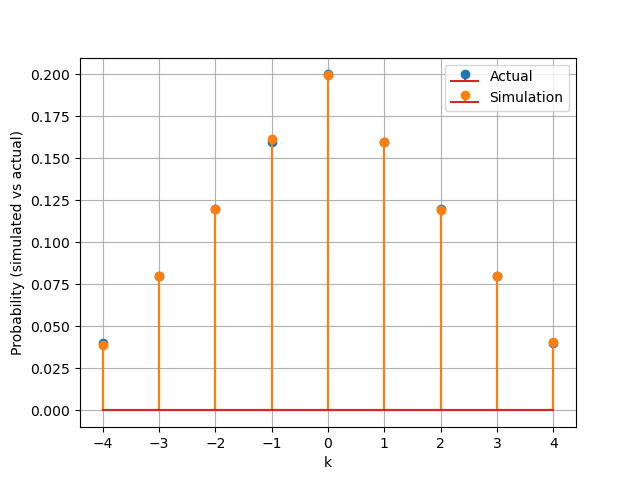
\includegraphics[width=\columnwidth]{./figs/fig.png}
\caption{Stem plot for P(Z)}
\label{fig:exemplar/12/13/3/1/}
\end{figure}
\end{document}

